\documentclass[hyperref=unicode,presentation,10pt]{beamer}

\usepackage[absolute,overlay]{textpos}
\usepackage{array}
\usepackage{graphicx}
\usepackage{adjustbox}
\usepackage[version=4]{mhchem}
\usepackage{chemfig}
\usepackage{caption}
\usepackage{makecell}

%dělení slov
\usepackage{ragged2e}
\let\raggedright=\RaggedRight
%konec dělení slov

\addtobeamertemplate{frametitle}{
	\let\insertframetitle\insertsectionhead}{}
\addtobeamertemplate{frametitle}{
	\let\insertframesubtitle\insertsubsectionhead}{}

\makeatletter
\CheckCommand*\beamer@checkframetitle{\@ifnextchar\bgroup\beamer@inlineframetitle{}}
\renewcommand*\beamer@checkframetitle{\global\let\beamer@frametitle\relax\@ifnextchar\bgroup\beamer@inlineframetitle{}}
\makeatother
\setbeamercolor{section in toc}{fg=red}
\setbeamertemplate{section in toc shaded}[default][100]

\usepackage{fontspec}
\usepackage{unicode-math}

\usepackage{polyglossia}
\setdefaultlanguage{czech}

\def\uv#1{„#1“}

\mode<presentation>{\usetheme{default}}
\usecolortheme{crane}

\setbeamertemplate{footline}[frame number]

\title[Crisis]
{Novinky v periodické tabulce prvků}

\author{Zdeněk Moravec, hugo@chemi.muni.cz \\ \adjincludegraphics[height=50mm]{img/IUPAC_PSP.jpg}}
\date{}

\begin{document}

\begin{frame}
	\titlepage
\end{frame}

\section{Úvod}
\frame{
	\frametitle{}
	\vfill
	\begin{columns}
		\begin{column}{.35\textwidth}
			\textbf{1869}
			\begin{figure}
				\adjincludegraphics[width=\textwidth]{img/1869-PSP.png}
				\caption*{Periodická tabulka prvků z roku 1869.\footnote[frame]{Zdroj: \href{https://commons.wikimedia.org/wiki/File:Mendeleev\%27s_1869_periodic_table.png}{Dmitrij Ivanovič Mendělejev/Commons}}}
			\end{figure}
		\end{column}
		\begin{column}{.65\textwidth}
			\textbf{2016}
			\begin{figure}
				\adjincludegraphics[width=\textwidth]{img/IUPAC_PSP.jpg}
				\caption*{Periodická tabulka prvků.\footnote[frame]{Zdroj: \href{https://iupac.org/what-we-do/periodic-table-of-elements/}{IUPAC}}}
				\end{figure}
		\end{column}
	\end{columns}
	\vfill
}

\section{Atom}
\subsection{Historický vývoj atomové teorie}
\frame{
	\frametitle{}
	\vfill
	\begin{columns}
		\begin{column}{.65\textwidth}
			\begin{itemize}
				\item Démokritos (460--370 př. n. l.) --- všechno jsoucí se skládá ze dvou prvků, „plného“ a „prázdného“, které do sebe nikdy nepřecházejí. „Plné“ tvoří nedělitelné (řecky atomoi) a nekonečně rozmanité částečky, které se pohybují v „prázdném“.
				\item Nedělitelnost atomu byla vyvrácena až v roce 1897 fyzikem J. J. Thompsonem, který objevil a charakterizoval elektron.\footnote[frame]{\href{https://isobelf.wordpress.com/wp-content/uploads/2013/08/falconer_corpusclestoelectrons_preprint.pdf}{Corpuscles to Electrons}}
			\end{itemize}
		\end{column}
		\begin{column}{.4\textwidth}
			\begin{figure}
				\adjincludegraphics[width=\textwidth]{img/Plum_pudding_atom.png}
				\caption*{Thompsonův pudinkový model atomu.\footnote[frame]{Zdroj: \href{https://commons.wikimedia.org/wiki/File:Plum_pudding_atom.svg}{Fastfission/Commons}}}
			\end{figure}
		\end{column}
	\end{columns}
	\vfill
}

\frame{
	\frametitle{}
	\vfill
	\begin{itemize}
		\item Niels Bohr (1885--1962) --- dánský fyzik, nositel Nobelovy ceny za fyziku z roku 1922.\footnote[frame]{\href{https://www.nobelprize.org/prizes/physics/1922/summary/}{The Nobel Prize in Physics 1922}}
		\item V letech 1911--1918 vytvořil tzv. \textit{Bohrův model atomu}.
		\item Zavedl tři postuláty:\footnote[frame]{\href{https://en.wikipedia.org/wiki/Bohr_model}{Bohr model}}
		\begin{enumerate}
			\item Atom je stabilní soustava složená z kladně nabitého jádra, v němž je soustředěna téměř celá hmotnost atomu, a z elektronového obalu. Elektrony obíhají kolem jádra po kružnicových drahách, na nichž nevyzařují žádnou energii.
			\item Atom se může nacházet pouze v kvantových stacionárních stavech s určitou hodnotou energie (na určitých energetických hladinách).
			\item Při přechodu mezi energetickými hladinami elektron absorbuje (při přechodu na hladinu s vyšší energií) nebo emituje (při přechodu na hladinu s nižší energií) právě jeden foton, jehož energie odpovídá energetickému rozdílu hladin.
		\end{enumerate}
	\end{itemize}
	\vfill
}

\frame{
	\frametitle{}
	\vfill
	\begin{figure}
		\adjincludegraphics[height=.65\textheight]{img/Bohr.png}
		\caption*{Bohrův model atomu.\footnote[frame]{Zdroj: \href{https://en.wikipedia.org/wiki/File:Atome_bohr_couches_electroniques_KLM.svg}{Cdang/Commons}}}
	\end{figure}
	\vfill
}

\subsection{Struktura atomu}
\frame{
	\frametitle{}
	\vfill
	\begin{columns}
		\begin{column}{.65\textwidth}
			\begin{itemize}
				\item Atom -- skládá se z elektronového obalu a atomového jádra
				\item Elektronový obal -- tvoří většinu objemu atomu, ale je skoro prázdný
				\item Atomové jádro -- malý objem, ale obsahuje většinu hmoty atomu
				\item Periodická tabulka prvků -- atomy (prvky) seřazené podle hmotnosti (počtu protonů)
				\item Perioda -- skupina prvků, které mají shodnou valenční slupku elektronového obalu
				\item Skupina -- prvky, které mají shodný počet elektronů ve valenční slupce
			\end{itemize}
		\end{column}
		\begin{column}{.4\textwidth}
			\begin{figure}
				\adjincludegraphics[width=\textwidth]{img/Sodium_Atom.png}
				\caption*{Model atomu sodíku.\footnote[frame]{Zdroj: \href{https://commons.wikimedia.org/wiki/File:Sodium_Atom.png}{Plazmi/Commons}}}
			\end{figure}
		\end{column}
	\end{columns}
	\vfill
}

\frame{
	\frametitle{}
	\vfill
	\begin{figure}
		\adjincludegraphics[height=.7\textheight]{img/Helium_atom_QM.png}
		\caption*{Model atomu helia; 1 pm = 10$^{-12}$ m; 1 fm = 10$^{-15}$ m.\footnote[frame]{Zdroj: \href{https://commons.wikimedia.org/wiki/File:Helium_atom_QM.svg}{Yzmo/Commons}}}
	\end{figure}
	\vfill
}

\subsection{Izotopy}
\frame{
	\frametitle{}
	\vfill
	\begin{itemize}
		\item Nuklid -- látka z atomů jednoho prvku, které mají stejný počet neutronů.
		\item Izotop -- konkrétní nuklid jednoho chemického prvku.
		\item Existenci izotopů prokázal v roce 1913 Frederick Soddy, který za tento objev získal v roce 1921 Nobelovu cenu za chemii.\footnote[frame]{\href{https://www.nobelprize.org/prizes/chemistry/1921/summary/}{The Nobel Prize in Chemistry 1921}}
	\end{itemize}
	\begin{figure}
		\adjincludegraphics[width=.7\textwidth]{img/Hydrogen-isotopes.png}
		\caption*{Izotopy vodíku.\footnote[frame]{Zdroj: \href{https://commons.wikimedia.org/wiki/File:Hydrogen_Deuterium_Tritium_Nuclei_Schmatic-en.svg}{Dirk Hünniger/Commons}}}
	\end{figure}
	\vfill
}

\subsection{Stabilita atomových jader}
\frame{
	\frametitle{}
	\begin{itemize}
		\item Na stabilitu má vliv velikost vazebné energie jádra a poměr mezi počtem protonů a neutronů. U lehkých jader je poměr zhruba 1:1, se vzrůstajícím protonovým číslem dochází ke zvyšování přebytku neutronů
		\item Nejvíce stabilních jader má protonové i neutronové číslo sudé, např.~\ce{^{12}_6C}, \ce{^{16}_8O}, ...
		\item Naopak kombinace lichého protonového a neutronového čísla je u stabilních jader vzácná, známe pouze čtyři: \ce{^1_1H}, \ce{^6_3Li}, \ce{^{10}_5B} a \ce{^{14}_7N}
		\item \textbf{Poločas rozpadu} - doba, za kterou dojde k rozpadu poloviny jader v systému
		\item Charakteristika nestabilních jader, pohybuje se od zlomků sekund až po milióny let
		\item $\frac{dN}{dt} = -\lambda N$
		\item $N(t) = N_0 e^{-\lambda t}$
		\item \scalebox{1.5}{$t_{\frac{1}{2}} = \frac{\ln 2}{\lambda} = \tau \ln 2$}
	\end{itemize}
}

\subsection{Radioaktivní rozpady}
\frame{
	\frametitle{}
	\begin{itemize}
		\item Pokud je v jádru nadbytek neutronů nebo protonů, jádro se přemění na stabilnější.
		\begin{itemize}
			\item $\alpha$ rozpad - rozpad charakteristický pro těžší jádra, dojde k uvolnění $\alpha$-částice (jádro \ce{^4_2He^{2+}}), vzniklé jádro má protonové číslo menší o 2 a~nukleonové o 4
			\item \ce{^{226}_{88}Ra -> ^{222}_{86}Rn + ^4_2He}
			\item V případě nadbytku neutronů může dojít k rozpadu neutronu na proton a elektron, během přeměny se uvolňuje částice $\beta^-$ ($^{\ 0}_{-1}$e$^-$)
			\item \ce{^{32}_{15}P -> ^{32}_{16}S + ^{\ \ 0}_{-1}e}
			\item V případě nadbytku protonů může dojít k rozpadu protonu na neutron a pozitron, během přeměny se uvolňuje částice $\beta^+$ ($^{\ 0}_{+1}$e$^+$)
			\item \ce{^{11}_{6}C -> ^{11}_{5}B + ^0_{+1}e}
			\item Nadbytek protonů v jádře může být kompenzován i pomocí \textit{elektronového záchytu}, kdy proton pohltí elektron a vznikne neutron
			\item \ce{^{7}_{4}Be + ^0_{-1}e -> ^{7}_{3}Li}
		\end{itemize}
	\end{itemize}
}

\subsection{Alotropie prvků}
\frame{
	\frametitle{}
	\vfill
	\begin{itemize}
		\item Koncept \textit{alotropie} navrhl v roce 1841 Jöns Jakob Berzelius, termín je odvozen z řeckého výrazu pro variabilitu.\footnote[frame]{\href{https://doi.org/10.1021/ed083p838}{The Origin of the Term Allotrope}}
		\item Alotropy prvku jsou rozdílné strukturní modifikace daného prvku, mají odlišné fyzikální i chemické vlastnosti.\footnote[frame]{\href{http://www.chemistryexplained.com/A-Ar/Allotropes.html}{Allotropes}}
		\item S alotropy se setkáváme např. u uhlíku, fosforu, síry a mnoha dalších prvků.
		\begin{itemize}
			\item \textit{Uhlík}:\footnote[frame]{\href{https://ksicht.natur.cuni.cz/aktualni-rocnik/}{KSICHT, seriál, ročník 2024/25}} diamant, grafit, grafen, fullereny, uhlíkové nanotrubice, $\ldots$
			\item \textit{Fosfor}: bílý, červený, černý, fialový
			\item \textit{Selen}: červený, šedý, černý
			\item \textit{Kobalt}: $\alpha$-kobalt, $\beta$-kobalt
		\end{itemize}
	\end{itemize}
	\begin{figure}
		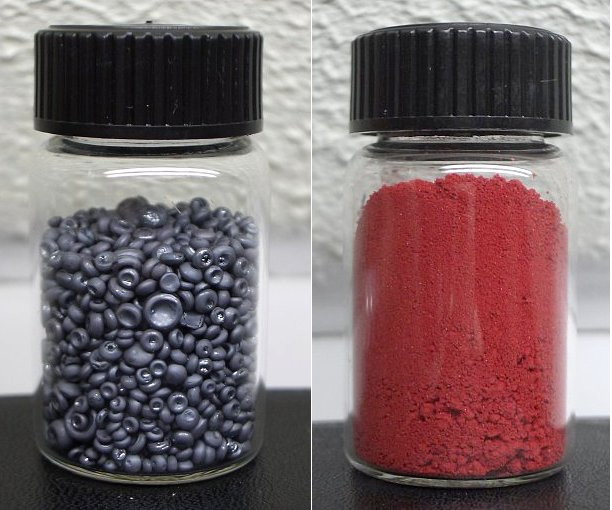
\includegraphics[height=.2\textheight]{img/SeBlackRed.jpg}
		\caption*{Černý a červený selen.\footnote[frame]{Zdroj: \href{https://commons.wikimedia.org/wiki/File:SeBlackRed.jpg}{W. Oelen/Commons}}}
	\end{figure}
	\vfill
}

\frame{
	\frametitle{}
	\vfill
	\begin{figure}
		\adjincludegraphics[height=0.7\textheight]{img/Eight_Allotropes_of_Carbon.png}
		\caption*{Allotropické modifikace uhlíku.\footnote[frame]{Zdroj: \href{https://commons.wikimedia.org/wiki/File:Eight_Allotropes_of_Carbon.png}{mstroeck/Commons}}}
	\end{figure}
	\vfill
}

\section{Současnost}
\frame{
	\frametitle{}
	\begin{figure}
		\adjincludegraphics[width=0.9\textwidth]{img/PSP-old.jpg}
		\caption*{PSP, stav před rokem 1997.\footnote[frame]{Zdroj: \href{https://commons.wikimedia.org/wiki/File:Periodic_Table_of_the_Elements_(46dcda15-95a8-4af0-a576-1f11c2274927).jpg}{NPGallery/Commons}}}
	\end{figure}
}

\frame{
	\frametitle{}
	\vfill
	\begin{figure}
		\adjincludegraphics[width=.95\textwidth]{img/IUPAC_PSP.jpg}
		\caption*{Periodická tabulka prvků, rok 2016.\footnote[frame]{Zdroj: \href{https://iupac.org/what-we-do/periodic-table-of-elements/}{IUPAC}}}
	\end{figure}
	\vfill
}

\subsection{Bismut}
\frame{
	\frametitle{}
	\vfill
	\textbf{Stabilita jader}
	\begin{columns}
		\begin{column}{.6\textwidth}
			\begin{itemize}
				\item Z prvních 82 prvků má 80 stabilní izotopy. Tc (43) a Pm (61) stabilní izotopy nemá.
				\item Z 251 známých stabilních izotopů se předpokládá, že 90 je opravdu stabilních a 161 má velice dlouhý poločas přeměny.
				\item U těžších prvků se neočekává, že by měly stabilní izotopy.
				\item V přírodě nacházíme 35 nuklidů, které mají poločas přeměny delší než je stáří Země (primordiální jádra).
				\item Nejdelší změřený poločas rozpadu má $^{128}$Te, 2,2$\times$10$^{24}$ let.
			\end{itemize}
		\end{column}

		\begin{column}{.55\textwidth}
			\begin{figure}
				\adjincludegraphics[width=.8\textwidth]{img/Isotopes_and_half-life.png}
				\caption*{Poločas přeměny izotopů.\footnote[frame]{Zdroj: \href{https://commons.wikimedia.org/wiki/File:Isotopes_and_half-life.svg}{BenRG/Commons}}}
			\end{figure}
		\end{column}
	\end{columns}
	\vfill
}

\frame{
	\frametitle{}
	\vfill
	\begin{itemize}
		\item Dlouho byl za stabilní (a zároveň nejtěžší stabilní jádro) považován izotop $^{209}$Bi, ale v roce 2003 bylo prokázáno, že se rozpadá za uvolnění částice $\alpha$.\footnote[frame]{\href{https://doi.org/10.1038/nature01541}{Experimental detection of alpha-particles from the radioactive decay of natural bismuth}}
		\item \ce{^{209}_{83}Bi -> ^{205}_{81}Tl + ^{4}_{2}$\alpha$}
		\item Poločas rozpadu je 2,01.10$^{19}$ let. Stáří vesmíru je odhadováno na 13,8$\times10^9$ let.
		\item Za nejtěžší stabilní jádro je nyní považováno jádro $^{208}_{\ 82}$Pb.
	\end{itemize}
	\begin{center}
		\begin{tabular}{|l|l|l|}
			\hline
			\textbf{Izotop} & \textbf{Poločas rozpadu} & \textbf{Typ rozpadu} \\\hline
			$^{207}$Bi & 31,55 let & $\beta^+$ \\\hline
			$^{208}$Bi & 3,7.10$^5$ let & $\beta^+$ \\\hline
			$^{209}$Bi & 2,01.10$^{19}$ let & $\alpha$ \\\hline
			$^{210}$Bi & 5,012 dne & $\beta^-$/$\alpha$ \\\hline
			$^{210m}$Bi & 3,04.10$^6$ let & $\alpha$ \\\hline
		\end{tabular}
	\end{center}
	\vfill
}

\subsection{Dokončení 7. periody}
\frame{
	\frametitle{}
	\textit{Supertěžké prvky} mají protonové číslo vyšší než 103.
	\begin{tabular}{|l|l|l|r@{ }l|}
		\hline
		\textbf{Protonové číslo} & \textbf{Značka} & \textbf{Název} & \multicolumn{2}{|c|}{\textbf{$T_{\frac{1}{2}}$}} \\\hline
		104 & Rf & Rutherfordium & 1,3 &h \\\hline
		105 & Db & Dubnium & 28 &h \\\hline
		106 & Sg & Seaborgium & 14 &min \\\hline
		107 & Bh & Bohrium & 11,5 &min \\\hline
		108 & Hs & Hassium & 110 &s \\\hline
		109 & Mt & Meitnerium & 67 &s \\\hline
		110 & Ds & Darmstadtium & 14 &s \\\hline
		111 & Rg & Roentgenium & 306 &s \\\hline
		112 & Cn & Copernicium & 28 &s\\\hline
		113 & Nh & Nihonium & 9,5 &s \\\hline
		114 & Fl & Flerovium & 19 &s \\\hline
		115 & Mc & Moscovium & 650 &ms \\\hline
		116 & Lv & Livermorium & 57 &ms \\\hline
		117 & Ts & Tennessine & 51 &ms \\\hline
		118 & Og & Oganesson &  181 &ms \\\hline
	\end{tabular}
}

\frame{
	\frametitle{}
	\vfill
	\begin{itemize}
		\item Organizace IUPAC vydala 9. 6. 2016 návrh na pojmenování nových čtyř prvků s protonovými čísly 113, 115, 117 a 118.\footnote[frame]{\href{https://iupac.org/iupac-is-naming-the-four-new-elements-nihonium-moscovium-tennessine-and-oganesson/}{IUPAC is naming the four new elements nihonium, moscovium, tennessine, and oganesson}}
		\item 28. 11. 2016 byly tyto názvy schváleny.\footnote[frame]{\href{https://iupac.org/iupac-announces-the-names-of-the-elements-113-115-117-and-118/}{IUPAC announces the names of the elements 113, 115, 117, and 118}}$^,$\footnote[frame]{\href{https://www.osel.cz/8881-dalsi-ctyri-supertezke-prvky-maji-sva-jmena.html}{Další čtyři supertěžké prvky mají svá jména}}
		\item Všechny tyto nově připravené prvky jsou nestabilní, jejich poločasy rozpadu se pohybují ve zlomcích sekund.
		\item Kromě metod přípravy, jsou studovány i jejich fyzikální a chemické vlastnosti.\footnote[frame]{\href{https://doi.org/10.1515/ract-2022-0015}{Five decades of GSI superheavy element discoveries and chemical investigation}}
	\end{itemize}
	\begin{tabular}{|c|c|c|}
		\hline
		\textbf{Protonové číslo} & \textbf{Původní název} & \textbf{Schválený název} \\
		\hline
		113 & Ununtrium (Uut) & Nihonium (Nh) \\
		\hline
		115 & Ununpentium (Uup) & Moscovium (Mc) \\
		\hline
		117 & Ununseptium (Uus) & Tennessine (Ts) \\
		\hline
		118 & Ununoctium (Uuo) & Oganesson (Og) \\
		\hline
	\end{tabular}
	\vfill
}

\subsubsection{Nihonium}
\frame{
	\frametitle{}
	\vfill
	\begin{itemize}
		\item \textit{Nihonium}
		\begin{itemize}
			\item Umělý prvek, protonové číslo 113, Nh.
			\item Poprvé byl připraven v roce 2003:
			\item \ce{^{243}_{95}Am + ^{48}_{20}Ca -> ^{291}_{115}Mc$^\star$ -> ^{288}_{115}Mc + 3 n -> ^{284}Nh + $\alpha$}
			\item \ce{^{243}_{95}Am + ^{48}_{20}Ca -> ^{291}_{115}Mc$^\star$ -> ^{287}_{115}Mc + 4 n -> ^{283}Nh + $\alpha$}
			\item \ce{^{286}_{113}Nh -> ^{282}_{111}Rg + $\alpha$}
		\end{itemize}
		\item Pojmenován byl po Japonsku -- „země vycházejícího slunce“.
		\item Známe osm izotopů $^{278}$Nh -- $^{290}$Nh, nejdelší poločas rozpadu má $^{286}$Nh, $t_\frac{1}{2}$ = 9,5~s.
		\item Chemické vlastnosti nihonia nebyly zatím detailně prozkoumány.\footnote[frame]{\href{https://arxiv.org/abs/1212.4292}{First foot prints of chemistry on the shore of the Island of Superheavy Elements}}
		\item Očekává se, že bude méně reaktivní než thallium a bude se podobat ušlechtilým kovům.
	\end{itemize}
	\vfill
}

\subsubsection{Moscovium}
\frame{
	\frametitle{}
	\vfill
	\textbf{Moscovium}
	\begin{itemize}
		\item Umělý prvek, protonové číslo 115, Mc.\footnote[frame]{\href{https://iupac.org/iupac-announces-the-names-of-the-elements-113-115-117-and-118/}{IUPAC announces the names of the elements 113, 115, 117, and 118}}
		\item Dřívější název tohoto prvku byl \textit{ununpentium}.
		\item Poprvé byl připraven v roce 2004:\footnote[frame]{\href{https://journals.aps.org/prc/abstract/10.1103/PhysRevC.69.021601}{Experiments on the synthesis of element 115}}
		\item \ce{^{243}_{95}Am + ^{48}_{20}Ca -> ^{288}_{115}Mc + 3 ^1_0n}
		\item \ce{^{243}_{95}Am + ^{48}_{20}Ca -> ^{287}_{115}Mc + 4 ^1_0n}
		\item Předpokládaná elektronová konfigurace: [Rn] 5f$^{14}$ 6d$^{10}$ 7s$^2$ 7p$^3$.
	\end{itemize}

	\begin{center}
		\begin{tabular}{|l|l|l|}
			\hline
			Izotop & Poločas rozpadu & Typ přeměny \\\hline
			$^{286}$Mc & 20 ms & $\alpha$ \\\hline
			$^{287}$Mc & 38 ms & $\alpha$ \\\hline
			$^{288}$Mc & 193 ms & $\alpha$ \\\hline
			$^{289}$Mc & 250 ms & $\alpha$ \\\hline
			$^{290}$Mc & 650 ms & $\alpha$ \\\hline
		\end{tabular}
	\end{center}
	\vfill
}

\subsubsection{Tennessin}
\frame{
	\frametitle{}
	\vfill
	\textbf{Tennessin}
	\begin{itemize}
		\item Umělý prvek, protonové číslo 117, Ts.\footnote[frame]{\href{https://iupac.org/iupac-announces-the-names-of-the-elements-113-115-117-and-118/}{IUPAC announces the names of the elements 113, 115, 117, and 118}}
		\item Název byl zvolen podle Tennessee (státu USA).\footnote[frame]{\href{https://www.ornl.gov/sites/default/files/Ts_Program\%20Final\%20sm.pdf}{The Discovery of Tennessine}}
		\item Poprvé byl připraven v dubnu 2010:\footnote[frame]{\href{https://doi.org/10.1103/PhysRevLett.104.142502}{Synthesis of a New Element with Atomic Number Z = 117}}
		\item \ce{^{249}_{97}Bk + ^{48}_{20}Ca -> ^{294}_{117}Ts + 3 ^1_0n}
		\item \ce{^{249}_{97}Bk + ^{48}_{20}Ca -> ^{294}_{117}Ts + 4 ^1_0n}
	\end{itemize}

	\begin{center}
		\begin{tabular}{|l|l|l|}
			\hline
			Izotop & Poločas rozpadu & Typ přeměny \\\hline
			$^{293}$Ts & 25 ms & $\alpha$ \\\hline
			$^{294}$Ts & 51 ms & $\alpha$ \\\hline
		\end{tabular}
	\end{center}
	\vfill
}

\subsubsection{Ogganesson}
\frame{
	\frametitle{}
	\begin{columns}
		\begin{column}{.6\textwidth}
			\vfill
			\textbf{Ogganesson}
			\begin{itemize}
				\item Umělý prvek, protonové číslo 118, Og.\footnote[frame]{\href{https://iupac.org/iupac-announces-the-names-of-the-elements-113-115-117-and-118/}{IUPAC announces the names of the elements 113, 115, 117, and 118}}
				\item Pojmenován byl podle ruského fyzika Yuri Ogganessiana, jde o druhý prvek pojmenovaný po žijící osobě.\footnote[frame]{\href{https://www.newscientist.com/article/mg23431210-600-up-and-atom-breaking-the-periodic-table/}{Mr Element 118: The only living person on the periodic table}}
				\item Poprvé byl připraven v roce 2002:\footnote[frame]{\href{https://www.washingtonpost.com/wp-dyn/content/article/2006/10/16/AR2006101601083.html}{Scientists Announce Creation of Atomic Element, the Heaviest Yet}}
				\item \ce{^{249}_{98}Cf + ^{48}_{20}Ca -> ^{294}_{118}Og + 3 ^1_0n}
			\end{itemize}

			\begin{center}
				\begin{tabular}{|l|l|l|}
					\hline
					Izotop & Poločas rozpadu & Typ přeměny \\\hline
					$^{294}$Og & 0,58 ms & $\alpha$ \\\hline
				\end{tabular}
			\end{center}
			\vfill
		\end{column}
		\begin{column}{.4\textwidth}
				\begin{figure}
				\adjincludegraphics[width=\textwidth]{img/Yuri_Oganessian.jpg}
				\caption*{Yuri Ogganessian.\footnote[frame]{Zdroj: \href{https://commons.wikimedia.org/wiki/File:Yuri_Oganessian.jpg}{VPRO/Commons}}}
			\end{figure}
		\end{column}
	\end{columns}
}

\section{Budoucnost}
\subsection{Hledání dalších supertěžkých prvků}
\frame{
	\frametitle{}
	\begin{columns}
		\begin{column}{.6\textwidth}
			\vfill
			\begin{itemize}
				\item Struktura atomového jádra je podobná struktuře elektronového obalu.
				\item Protony mají svůj systém hladin, stejně tak neutrony. Z toho důvodu existují velmi stabilní kombinace počtu protonů a neutronů, tzv. \textit{magická čísla}, kdy jsou tyto slupky zcela zaplněny.
				\item 2, 8, 20, 28, 50, 82, 126\footnote[frame]{\href{https://oeis.org/A018226}{Magic numbers of nucleons}}
				\item U těchto číselných kombinací se očekává zvýšená stabilita jader.
				\item Stabilitu jader dále zvyšuje sudý počet protonů i neutronů.
			\end{itemize}
			\vfill
		\end{column}
		\begin{column}{.4\textwidth}
			\begin{figure}
				\adjincludegraphics[height=0.6\textheight]{img/Table_isotopes_en.png}
				\caption*{Typ rozpadu jádra v závislosti na protonovém čísle.\footnote[frame]{Zdroj: \href{https://commons.wikimedia.org/wiki/File:Table_isotopes_en.svg}{Napy1kenobi/Commons}}}
			\end{figure}
		\end{column}
	\end{columns}
}

\frame{
	\frametitle{}
	\vfill
	\begin{itemize}
		\item V oblasti okolo magických čísel se očekávají tzv. \textit{ostrovy stability}.\footnote[frame]{\href{https://www.osel.cz/11733-novinky-ve-studiu-velmi-tezkych-a-supertezkych-prvku.html}{Novinky ve studiu velmi těžkých a supertěžkých prvků}}
		\item Přesnou polohu těchto ostrovů je obtížné určit, každé nově objevené jádro pomáhá zpřesnit modely.\footnote[frame]{\href{http://www.chemicke-listy.cz/ojs3/index.php/chemicke-listy/article/view/3334}{Meze periodické tabulky}}
		\item První ostrov stability se předpokládá v blízkosti jádra $^{298}_{114}$Fl.
		\item Příprava těchto jader je ovšem velmi komplikovaná, např.:
		\item \ce{^{248}_{94}Pu + ^{50}_{20}Ca -> ^{298}_{114}Fl}
		\item \ce{^{248}_{96}Cm + ^{238}_{92}U -> ^{298}_{114}Fl + ^{186}_{74}W + 2 ^1_0n}
		\item Druhý ostrov stability se předpokládá až u protonového čísla 164, to je ale se současnou technologií nedosažitelné.\footnote[frame]{\href{https://doi.org/10.1007/BF01406719}{Investigation of the stability of superheavy nuclei around Z=114 and Z=164}}
	\end{itemize}
	\vfill
}

\frame{
	\frametitle{}
	\vfill
	\begin{figure}
		\adjincludegraphics[height=0.65\textheight]{img/Island_of_Stability.png}
		\caption*{Ostrovy stability.\footnote[frame]{Zdroj: \href{https://commons.wikimedia.org/wiki/File:Island_of_Stability.svg}{	InvaderXan/Commons}}}
	\end{figure}
	\vfill
}

\frame{
	\frametitle{}
	\vfill
	\begin{itemize}
		\item Nová supertěžká jádra lze produkovat několika způsoby:\footnote[frame]{\href{https://www.osel.cz/8666-jak-se-produkuji-a-studuji-supertezke-prvky.html}{Jak se produkují a studují supertěžké prvky}}
		\begin{enumerate}
			\item Ostřelováním těžkých jader intenzivním proudem neutronů, např.:
			\begin{itemize}
				\item \ce{^{238}_{92}U + ^1_0n -> ^{239}_{92}U ->[23 min] ^{239}_{93}Np + $\beta^-$ ->[56 hod] ^{239}_{94}Pu + $\beta^-$}
			\end{itemize}
			\item Ostřelováním terče s obsahem těžkých, stabilních jader jiným těžkým jádrem.
			\begin{itemize}
				\item \ce{^{64}_{28}Ni + ^{209}_{83}Bi -> ^{272}_{111}Rg + ^1_0n}
				\item \ce{^{70}_{30}Zn + ^{208}_{82}Pb -> ^{277}_{112}Cn + ^1_0n}
			\end{itemize}
		\end{enumerate}
		\item Výzkum nových prvků probíhá v několika laboratořích:
		\begin{itemize}
			\item Joint Institute for Nuclear Research v Dubně\footnote[frame]{\href{http://www.jinr.ru/main-en/}{Joint Institute for Nuclear Research}}
			\item Riken v Japonsku\footnote[frame]{\href{https://www.riken.jp/en/}{RIKEN}}
			\item GSI Helmholtz Centre for Heavy Ion Research v Darmstadtu\footnote[frame]{\href{https://www.gsi.de/start/aktuelles.htm}{GSI}}
		\end{itemize}
	\end{itemize}
	\vfill
}

\frame{
	\frametitle{}
	\vfill
	\begin{itemize}
		\item Syntéza prvních prvků 8. periody je již studována.
		\item \textbf{Ununennium}, Uue, prvek 119
		\begin{itemize}
			\item První neúspěšný pokus byl proveden již v roce 1985\footnote[frame]{\href{https://doi.org/10.1103/PhysRevC.32.1760}{Search for superheavy elements using the $^{48}$Ca+$^{254}$Es$^g$ reaction}}
			\item \ce{^{254}_{99}Es + ^{48}_{20}Ca -> ^{302}_{119}Uue^*}
			\item Nadějnější se zdá experiment z roku 2020 (Riken, Japonsko):\footnote[frame]{\href{https://www.nature.com/articles/d41586-019-00285-9}{Extreme chemistry: experiments at the edge of the periodic table}}
			\item \ce{^{248}_{96}Cm + ^{51}_{23}V -> ^{299}_{119}Uue^*}
		\end{itemize}
		\item \textbf{Unbibium}, Ubb, prvek 122
		\begin{itemize}
			\item V roce 2000 se o syntézu pokoušeli v GSI:\footnote[frame]{\href{https://doi.org/10.1103/PhysRevC.98.024308}{Investigations of the synthesis of the superheavy element Z = 122}}
			\item \ce{^{238}_{92}U + ^{65}_{29}Cu -> ^{303}_{121}Ubu^*}
		\end{itemize}
		\item Cesta k těžším prvkům zatím není zcela zřejmá.
		\item Jednou z exotičtějších možností je studium prvků vyvržených během exploze supernovy.\footnote[frame]{\href{https://www.scientificamerican.com/article/superheavy-elements-are-breaking-the-periodic-table/}{Superheavy Elements Are Breaking the Periodic Table}}
	\end{itemize}
	\vfill
}


\section{Závěr}
\frame{
	\vfill
	\centering \Huge
	\textbf{Děkuji za pozornost} \\[2ex]

	\large
	Zdeněk Moravec\\
	hugo@chemi.muni.cz \\
	\vfill
}

\end{document}